\chapter{Modellierung des Wasserstoff-Energiesystems}
\label{cha:Methode}
Im folgende Kapitel wird die Modellierung des Wasserstoff-Energiesystems dokumentiert.
Dazu werden Anfangs die Modelle des Elektrolyseurs und der Brennstoffzelle vorgestellt. Weiterhin werden Bewertungskriterien für Konzepte des Wasserstoff-Energiesystems ausgearbeitet und anschließend alternative Systemkonzepte präsentiert. 
Im letzten Abschnitt werden die für die Simulation der Konzepte gewählten Parameter und Randbedingungen hergeleitet.

\section{Implementierung der Wasserstoffkomponenten in Modelica} 
Für die Simulations-gestützte Bewertung der Wasserstoff-Energiesysteme ist ein Modell erforderlich, welches das Verhalten der gesamten Elektrolyseur-Anlage beschreibt. Dazu werden zusätzlich zur Elektrolyse-Zelle die relevanten Systemkomponenten in der Modellierung berücksichtigt. Um die Wiederverwendbarkeit des Modells zu verbessern werden als Eingangsgrößen Kennwerten aus Datenblättern verwendet und wo nötig um Literaturangaben erweitert. Der Fokus liegt dabei auf der Modellierung von alkalischen- und PEM-Zellen, da sie, wie in \ref{subsec:Technologien der Wasserelektrolyse} sowie \ref{subsec:BZ}, erläutert der aktuelle Standard sind. Es ist ein Detaillierungsgrad angestrebt, der einerseits ein ausreichend genaue Modellierung für die Bewertung der Wasserstoff-Energiesysteme ermöglicht und andererseits zu einer akzeptablen Rechen- und Entwicklungszeit führt.
Weiterhin wird der Wärmehaushalt der Brennstoffzelle zur Beschreibung der Kraft-Wärme-Kopplung modelliert.\\

Nach \citet{schamai_modelica_2009} ist \textit{Modelica} ideal für die Modellierung von physikalischen Systemen mit Energieaustausch und weiteren zeitkontinuierlichen Vorgängen geeignet. Zu diesen Systemen zählen auch die Wasserstoff-Energiekonzepte, die in dieser Arbeit untersucht werden. \textit{Modelica} ist eine objektorientierte Sprache, mit deren Hilfe Systeme durch gewöhnliche Differentialgleichungen in Kombination  mit diskreten Vorfällen beschrieben werden. Das Modell wurde in Modelica 4.0.0 in der Entwicklungsumgebung Dymola 2021x entwickelt.\\

\subsection{Modellierung der Elektrolysezelle}
\label{subsec:Modellierung der Zelle}
In Abbildung \ref{fig:Modellstruktur} ist die gewählte Modellarchitektur graphisch dargestellt. Das partielle Modell wird verwendet, da die Beschreibung der idealen Zellspannung und die Approximationen der Verlustmechanismen für Elektrolyseur und Brennstoffzelle identisch sind.
 
\begin{figure}[h]
	\centering
		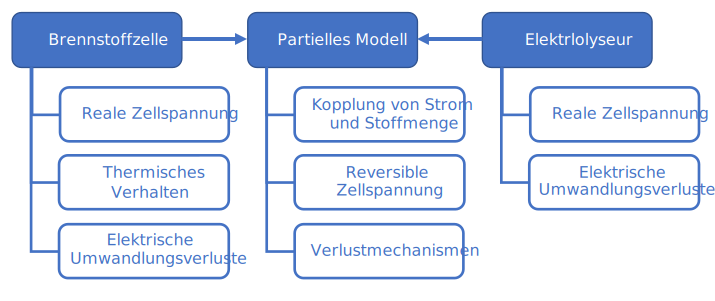
\includegraphics[scale=1]{Figures/Modellstruktur}
		\caption{Architektur des entwickelten Elektrolyseur- und Brennstoffzellen-Modells.}
\label{fig:Modellstruktur}	
\end{figure}

Im partiellen Modell sind daher daher folgende Zusammenhänge implementiert: Der Zusammenhang von Strom und produzierter Stoffmenge (Gleichung \ref{gl:n_i}), die Gleichungen zur Berechnung der idealen Zellspannung (Gleichung \ref{gl:Urev} sowie der Temperatur- und Druckeinfluss) und die Berechnung der Aktivierungsverluste  (Gleichung  \ref{gl:Akt}) und Ohmschen Überspannungen (für PEM-Zellen Gleichung \ref{gl:Ohm2}, sonst \ref{gl:Ohm}). Über den \textit{Bauart}-Parameter wird im Modell die Technologie der Zelle ausgewählt.
Für die drei in \ref{subsec:Technologien der Wasserelektrolyse} beschriebenen Bauarten sind im Modell verschiedene Werte für die Austauschstromdichte ($i_0$), den Durchtrittsfaktor ($\alpha$), den Elektrodenabstand ($\delta$) und die Leitfähigkeit ($\sigma$) hinterlegt. Abhängig vom \textit{Bauart}-Parameter werden diese zur Berechnung der Verluste genutzt.\\

Die Modelle für Elektrolyseur und Brennstoffzelle enthalten die Gleichungen zur Berechnung der realen Zellspannung (Gleichung \ref{gl:U_realEL} beziehungsweise \ref{gl:U_real-BZ}) sowie die Approximationen der in \ref{subsec:Systemkomponenten} erläuterten Umwandlungsverluste. Diese werden im Modell als über den Betriebsbereich konstant angenommen. Das erweist sich unter Beachtung des von \citet[S.~50]{tjarks_pem-elektrolyse-systeme_2017} angeführten Verlaufs des Wirkungsgrades eines Gleichrichters insbesondere im oberen Lastbereich als akzeptable Näherung. Auch auf den von \citet{trubitsyn_high-efficiency_2010} untersuchten Wechselrichter trifft diese Aussage zu.\\

Das Brennstoffzellenmodell enthält darüber hinaus die Berechnung der zur Verfügung stehenden Abwärme. Die Anfahrzeit von Elektrolysezellen liegt aus dem Stand-by nach \citet{milanzi_technischer_2018} bei $10-\SI{30}{\s}$, was im Vergleich zu den für die Simulation verwendeten Zeitschritten ($\SI{900}{\s}$) als vernachlässigbar angenommen wird. Daher werden im Rahmen dieser Arbeit dynamische Vorgänge, die insbesondere durch die  Betriebstemperatur der Zelle beeinflusst werden \citep{garcia-valverde_simple_2012}, nicht betrachtet.\\
Zur Modellierung des thermischen Verhaltens wird somit vereinfachend angenommen, dass die Betriebstemperatur stets konstant ist. Daher wird die Energiebilanz aus \ref{gl:Energiebilanz} wie folgt vereinfacht:

\begin{align}
0 = (\dot{n}_{H2} \cdot c_{p, H2} + \dot{n}_{Luft} \cdot c_{p, Luft}) \cdot (T_{Umgebung} - T) + I \cdot (U_{tn} - U_{Zelle}) - \dot{Q}
\end{align}

Der Wärmestrom $\dot{Q}$ setzt sich aus den Wärmeverlusten $\dot{Q}_{Verlust}$ und der nutzbaren Abwärme $\dot{Q}_{Nutz}$ zusammen. Die Wärmeverluste werden über den Wärmeverlustfaktor $C_{th}$ bestimmt:

\begin{align}
\dot{Q}_{Verlust} = C_{th} \cdot (T - T_{Umgebung}) 
\end{align}

Die zur Deckung des Heizwärmebedarfs genutzte Abwärme der Brennstoffzelle, wird im Modell in Gaseinsparungen umgerechnet. Angenommen wird dafür, dass der Wirkungsgrad der Gasheizung bei $\SI{90}{\%}$ liegt (\citet{herrmann_effizienz_2006} gibt für Gasheizungen einen Bereich von $80$ bis $\SI{110}{\%}$ an).\\ 

\section{Entwicklung von Energiesystem-Konzepten}
Im folgenden Abschnitt werden anfangs die zur Bewertung der Systemkonzepte genutzten Kriterien erläutert. Zudem werden die betrachteten Konzepte sowie die gewählte Betriebsstrategie erläutert. Weiterhin wird das aktuelle System sowie die betrachteten Erweiterungen beschrieben. Abschließend werden die gewählten Parameter und Randbedingungen angeführt.

\subsection{Identifikation sinnvoller Bewertungskriterien}
In \citet{reich_grundlagen_2018} werden Kriterien zum Vergleich von Energiesystemen angeführt, die eine umfassende Bewertung ermöglichen. Als für ein Unternehmen relevante Kriterien werden in dieser Arbeit Kennwerte zur ökonomische sowie ökologische Bewertung der Konzepte genutzt.\\

Zur ökonomischen Bewertung wird der Kapitalwert - eine Kennzahl der Dynamischen Investitionsrechnung \citep{muller_vorlesung_2020} - als Kriterium verwendet . 
Fällt der Kapitalwert einer Investition positiv aus, so wird diese als wirtschaftlich sinnvoll bewertet. Der Kapitalwert $C$ für einen Zeitraum von $n$ Jahren errechnet sich nach Gleichung \ref{gl:Kapitalwert} aus den Anfangsinvestitionen $I_0$, den jährlichen Einsparungen $Z_{ein}$ und Ausgaben $Z_{aus}$ und dem kalkulatorischen Zinssatz $r$ \citep{muller_vorlesung_2020} (Die jährlichen Einsparungen ergeben sich in dieser Arbeit aus den verminderten Strom- und Gaskosten und der Einspeisevergütung und als Ausgaben werden zusätzliche Wartungskosten gewertet):

\begin{align}
C = -I_0 + \frac{(1+r)^n-1}{(1+r)^n \cdot r} \cdot (Z_{ein} - Z_{aus})
\label{gl:Kapitalwert}
\end{align}

Als ökologisches Bewertungskriterium dient in dieser Arbeit der eingesparte \ce{CO2}-Ausstoß ($\Delta m_{\ce{CO2}}$) nach Gleichung \ref{gl:CO2}. Dieser setzt sich einerseits aus den Stromeinsparung $\Delta P_{el}$ in Verbindung mit dem \ce{CO2}-Faktor für den Strommix ($f_{Strom}$) und andererseits aus den Gaseinsparungen ($\Delta Q$) und dem \ce{CO2}-Faktor des Erdgases ($f_{Gas}$) zusammen. Als Stromeinsparungen werden in dieser Arbeit neben dem eingesparten Netzverbrauch auch die Einspeisung gewertet. Die \ce{CO2}-Faktor geben die Emissionen in 
\si{\g_{CO2}\per\kiloWh} an.
Für eine gesamtheitliche Betrachtung werden auch die \ce{CO2}-Emissionen miteinbezogen, die bei der Produktion der Komponenten entstehen, um die das Wasserstoff-Energiesystem erweitert wird ($\Delta m_{Prod.}$). 

\begin{align}
\Delta m_{\ce{CO2}} = \Delta P_{el} \cdot f_{Strom} + \Delta Q \cdot f_{Gas} - \Delta m_{Prod.}
\label{gl:CO2}
\end{align}

\subsection{Systemkonzepte}

\begin{figure}[h]
	\centering
		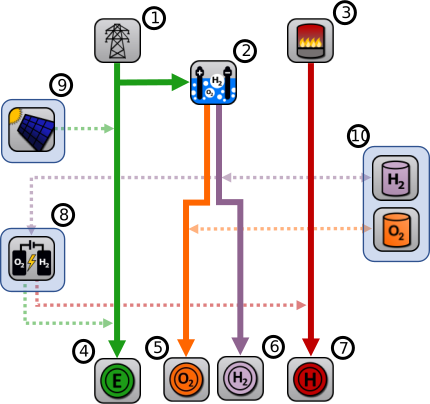
\includegraphics[scale=1]{Figures/Systemkonzepte}
		\caption{Aktuelles System sowie betrachtete Erweiterungen (1.Netzanschluss 2.Elektrolyseur 3.Gasheizung 4.Strombedarf 5.Wasserstoffbedarf 6.Sauerstoffbedarf 7.Heizwärmebedarf - Erweiterungen: 8.Brennstoffzelle 9.PV-Anlage 10.Gasspeicher).}
\label{fig:Modellstruktur}	
\end{figure}

In Abbildung \ref{fig:Modellstruktur} wird das aktuelle Wasserstoff-Energiesystem, sowie die in dieser Arbeit berücksichtigten Systemkonzepte dargestellt. Folgende Anforderungen werden dabei an die Systemkonzepte gestellt:
Der Strombedarf(4) und Heizwärmebedarf(6) muss gedeckt werden und die zum Betrieb der Veredelungsanlagen benötigte Menge an Sauerstoff(5) und Wasserstoff(6) muss bereitgestellt werden. 
Im aktuellen System wird der Strom aus dem Netz(1) bezogen, der Wärmebedarf von einer Gasheizung(3) gedeckt und die Prozessgase von einem alkalischen Elektrolyseur(2) produziert.\\

Als Erweiterung werden 4 Konzepte in betrachtet, die in Tabelle \ref{tb:Konzepte} aufgelistet sind. Bei Konzept 1 wird das bestehende System um eine Brennstoffzelle(8) erweitert, die den Wasserstoffüberschuss zur Kraft-Wärme-Kopplung nutzt. Beim zweiten Konzept wird die Verwendung einer PV-Anlage(9) betrachtet - Konzept 3 enthält sowohl eine PV-Anlage als auch eine Brennstoffzelle. Konzept 4 beinhaltet die Erweiterung mit einer PV-Anlage in Kombination mit einem Gasspeicher(10).

\begin{table}[ht]
		\centering
		\caption{In der Simulationsstudie betrachtete Erweiterungen des Wasserstoff-Energiesystems.}
		\begin{tabular}{l c}
		\toprule
		 & Erweiterungen\\	
		\midrule
		Konzept 1 & Brennstoffzelle\\
		Konzept 2 & PV-Anlage\\
		Konzept 3 & Brennstoffzelle und PV-Anlage\\
		Konzept 4 & PV-Anlage und Gasspeicher\\
		\bottomrule
		\end{tabular}
		\label{tb:Konzepte}
\end{table}	
   
Konzepte 1-3 werden Bedarfs-gesteuert betrieben, was auch der Betriebsstrategie im aktuellen System entspricht. Bei Konzept 4 wird im Falle von Solarstrom-Überschuss eine Einspeicherung in Form von Prozessgasen vorgenommen. Sobald der Solarstrom nicht ausreicht, um die Produktionsstätte samt Elektrolyseur zu versorgen, werden, falls vorhanden, die im Speicher gelagerten Gase den Anlagen zugeführt.

\subsection{Parametrierung der Komponenten}
Im folgenden Abschnitt werden die gewählten Parameter zur Simulation der Systemkonzepte vorgestellt. Dies beinhaltet einerseits die Parametrierung der Wasserstoffkomponenten als auch der PV-Anlage.

\paragraph{Alkalischer Elektrolyseur}\ \\
Im betrachteten System ist ein alkalischer Elektrolyseur vom Hersteller ErreDue S.p.A. mit der Modellbezeichnung G-32 verbaut. Als voreingestellte Betriebstemperatur ist $\SI{60}{\degreeCelsius}$ angegeben und der Betriebsdruck liegt standardmäßig bei $\SI{4}{\bar}$.
Für die gesamte Zellfläche liegen keine Angaben vor, daher wird diese anhand der maximal produzierten Stoffmenge und den Literaturangaben zur maximalen Stromdichte von alkalischen Elektrolyseuren abgeschätzt. Die Berechnung dazu ist im Anhang \ref{Apx:Modelle} aufgeführt. Als Elektrolyt dient 20-prozentige Natronlauge, was einer Stoffmengenkonzentration von $\SI{6,095}{\mol\per\l}$ entspricht \citep{periodensystem-online_dichtewerttabelle_nodate-1}.
Für den Elektrodenabstand ($\delta_{alk}$), den Durchtrittsfaktor ($\alpha$) und die Austauschstromdichte ($i_0$) werden die von \citet{milewski_modeling_2014} angegebenen Werte übernommen (s. \ref{Apx:Modelle}). 
Der Wirkungsgrad des Gleichrichters wird in dieser Arbeit mit $\SI{95}{\%}$ angenommen. Grundlage dafür ist der von \citet[S.~50]{tjarks_pem-elektrolyse-systeme_2017} abgebildete Verlauf des Wirkungsgrads eines Gleichrichters über der Leistung. In einem Leistungsbereich von $20-\SI{100}{\%}$ liegt der Wirkungsgrad zwischen $94-\SI{96}{\%}$.

\begin{table}[htb]
		\centering
		\caption{Zur Simulation des alkalischen Elektrolyseurs verwendete Parameter.}
		\begin{tabular}{l c c}
		\toprule
		Betriebstemperatur & $T$ & $\SI{60}{\degreeCelsius}$\\
		Betriebsdruck & $p$ & $\SI{4}{\bar}$\\
		Gesamtfläche & $A_{ges}$ & $\SI{10,2}{\m\squared }$\\
		Elektrolytkonzentration & $m$ & $\SI{6,095}{\mol \per \l}$\\
		Austauschstromdichte & $i_0$ & $ \SI{3,15}{\A\per\m\squared}$\\
		Durchtrittsfaktor & $\alpha$ & $\SI{0,17}{}$\\
		Elektrodenabstand & $\delta_{alk}$ & $\SI{0,66}{\cm}$\\
		Effizienz des Gleichrichters & $\eta_{GR}$ & $\SI{95}{\%}$ \\
		\bottomrule
		\end{tabular}
		\label{tb:ParameterElektrolyseur}
\end{table}	

\paragraph{PEM-Brennstoffzelle}\ \\
Weil PEM-Zellen - wie in \ref{subsec:BZ} angeführt - die meist verwendete Bauart bei Brennstoffzellen sind, wird diese Bauart für die Systemkonzepte ausgewählt. Für die Betriebstemperatur werden $\SI{80}{\degreeCelsius}$ angenommen und für den Betriebsdruck wird der Wert des Elektrolyseurs verwendet. Die Zellfläche ist so gewählt, dass die maximal produzierte Stoffmenge des Elektrolyseurs der maximal verwendeten Stoffmenge der Brennstoffzelle gleicht (siehe \ref{Apx:Modelle}). \citet{rashid_hydrogen_2015} nennen $100-\SI{200}{\micro\m}$ als übliche Membrandicke, daher ist diese im Modell mit $\SI{150}{\micro\m}$ abgeschätzt.
Die Werte der Parameter $i_0$, $\alpha$ und $C_{th}$ sind aus der Arbeit von \citet{webster_implementation_2019} entnommen, der Wärmeverlustfaktor $C_{th}$ wird anhand der Zellfläche skaliert, um den Einfluss der Baugröße auf die Konvektionsfläche zu berücksichtigen (siehe \ref{Apx:Modelle}). 
Der Wirkungsgrad des Wechselrichters wird auf Grundlage der von \citet{trubitsyn_high-efficiency_2010} vorgestellten Daten mit $\SI{96}{\%}$ angenommen.

\begin{table}[ht]
		\centering
		\caption{Zur Simulation der PEM-Brennstoffzelle verwendete Parameter.}
		\begin{tabular}{l c c}
		\toprule
		Betriebstemperatur & $T$ & $\SI{80}{\degreeCelsius}$\\
		Betriebsdruck & $p$ & $\SI{4}{\bar}$\\
		Gesamtfläche & $A_{ges}$ & $\SI{2,55}{\m\squared }$\\
		Membrandicke & $\delta_{pem}$ & $\SI{150}{\micro\m}$\\
		Austauschstromdichte & $i_0$ & $ \SI{2,16e-4}{\A\per\m\squared}$\\
		Durchtrittsfaktor & $\alpha$ & $0,7353$\\
		Elektrischer Widerstand & $R_{ele}$ & $\SI{0,096}{\ohm\per\cm\squared}$ \citep{tjarks_pem-elektrolyse-systeme_2017}\\	
		Wärmeverlustfaktor & $C_{th}$ & $\SI{21,939}{\W\per\K}$\\
		Effizienz des Wechselrichters & $\eta_{WR}$ & $\SI{96}{\%}$ \\
		\bottomrule
		\end{tabular}
		\label{tb:ParameterBrennstoffzelle}
\end{table}	

\paragraph{PV-Anlage}\ \\
Als PV-Anlage wird das Modell SE6M60-Series des Herstellers Symphony Energy in der Ausführung SE-M215 verwendet \citep{symphony_energy_coltd_se6m60_nodate}. Ein Simulationsmodell dafür ist in der Aixlib bereits implementiert. Die Peakleistung eines Moduls beträgt $\SI{215}{\W}$ bei einer Fläche von $\SI{1,44}{\m\squared}$. Auf der verfügbaren Dachfläche des Quarzglasherstellers ($\SI{537}{\m\squared}$) könne somit maximal 372 Module platziert werden. Daraus ergibt sich eine Peakleistung der Anlage von $\SI{79,98}{\kilo\W}$.\\
Für die Wetterdaten werden Messwerte aus dem Jahr 2020 verwendet. Der Temperaturverlauf ist der Datenbank des Deutschen Wetterdienstes (DWD) entnommen \citep{dwd_historische_nodate} und für die Einstrahlzahlen werden Instituts-eigene Messungen verwendet. Aufgrund fehlender Daten in den Aufzeichnungen des Instituts wurden für die Monate Januar und Februar die von der DWD angegebenen Werte für ein mittleres Testreferenzjahr 2015 verwendet \citep{dwd_klimaberatungsmodul_nodate}.

\subsection{Randbedingungen}
Randbedingungen der Simulationen sind die Bedarfsverläufe von Strom, Heizwärme und Prozessgasen.\\

Für den Strombedarf wird in der Simulation der gemessene Verbrauch des Quarzglasherstellers im Jahr 2020 verwendet. Weil der Elektrolyseur im Jahr 2020 in den Monaten März bis September nicht im Betrieb war, wird in diesem Zeitraum der simulierte Bedarf des Elektrolyseurs zum gemessenen Stromverbrauch addiert.\\

Der Heizwärmebedarf wird aus dem Gasverbrauch des Quarzglasherstellers im Jahr 2020 abgeschätzt. Neben der Gasheizung verbrauchen weitere Anlagen Erdgas. Der Gasbedarf der weiteren Verbraucher wird auf Grundlage der Sommermonate überschlagen, denn für die Monate Juni bis August wird angenommen, dass kein Heizbedarf vorliegt (Ausführlicher beschrieben in \ref{Apx:Systemkonzepte}).\\

Für den Wasserstoff- und Sauerstoffbedarf werden zwei Datensätze genutzt, welche aus den Einkaufsmengen der Gase vor Anschaffung des Elektrolyseurs bestimmt wurden (siehe auch \ref{Apx:Systemkonzepte}). Im Datensatz der sich nach den Verbrauchswerten aus 2018 richtet, wird angenommen, dass Werktags für $\SI{4}{\hour},\SI{30}{\minute}$ Wasserstoff und für $\SI{7}{\hour},\SI{15}{\minute}$ Sauerstoff benötigt wird. Der angenommene Stoffmengenstrom liegt bei durchschnittlich $\SI{75}{\%}$ der Maximalleistung des Elektrolyseurs. Die Daten werden zur Steigerung der Realitätsnähe mit einem Rauschen behaftet, wodurch der Bedarf beim Betrieb zwischen $50$ und $\SI{100}{\%}$ schwankt. Es ergibt sich im Vergleich zum realen Jahresverbrauch aus 2018 für den Wasserstoffbedarf eine Abweichung von $\SI{1,5}{\%}$ und für den Sauerstoffbedarf eine Abweichung von $\SI{0,2}{\%}$. In Abbildung \ref{fig:Daten1} ist ein exemplarischer Tagesverlauf ds Datensatzes dargestellt. 

\begin{figure}[h]
	\centering
		\includegraphics[scale=1]{Figures/Datensatz1molar}
		\caption{An 2018 angelehnter, exemplarischer Verlauf des Wasserstoff- und Sauerstoffbedarfs über einen Arbeitstag.}	
\label{fig:Daten1}	
\end{figure}

Bei dem Datensatz für 2019 wird angenommen, dass tägliche für $\SI{2}{\hour},\SI{45}{\minute}$ Wasserstoff und für $\SI{4}{\hour}$ Sauerstoff benötigt wird. Daraus ergeben sich im Vergleich zum realen Jahresverbrauch von 2019 Abweichungen von $\SI{0,7}{\%}$ beim Sauerstoffbedarf und $\SI{0,5}{\%}$ beim Wasserstoffbedarf. Ein exemplarischer Tagesverlauf des Datensatzes ist in Abbildung \ref{fig:Daten2} dargestellt.

\begin{figure}[h]
	\centering
		\includegraphics[scale=1]{Figures/Datensatz2molar}
		\caption{An 2019 angelehnter, exemplarischer Verlauf des Wasserstoff- und Sauerstoffbedarfs über einen Arbeitstag.}		
\label{fig:Daten2}	
\end{figure}